\section{flow optimizations}
\label{sec:flowOpt}

We carried out most of the optimization studies with another analysis configuration using a transformer architecture for the massplane definition \hl{need references to a couple of my pairAGraph talks}. Also, we did most of the optimization modeling 2b instead of the 4b validation regions since while the standard 4b analysis was still in flux, we didn't want to have any of our optimization studies use any part of the SR before the analysis was frozen and unblinded. 

\subsection{Modelling variables}
\label{subsec:hp-varOpt}

\begin{figure}
\centering
\subfloat[Real NVP modeling HH variables]{
	\includegraphics[width=0.44\textwidth]{{figures/flows/rnvp_log_m_hh_cor2_absCosThetaStar_5_layers_H_16_lr_0.001_0.001_iter0/m_hh_cor2_SR_mean_1sigma_250seeds_log.pdf}}
	}
\subfloat[Real NVP modeling HC variables]{
	\includegraphics[width=0.44\textwidth]{{figures/flows/data16_PFlow-FEB20-5jets_SM_2b_p_0.01_2b_detaCut/rnvp_log_pT_h1_log_pT_h2_eta_h2_eta_h1_log_dphi_hh_5_layers_H_32_lr_0.001_0.001_iter0/m_hh_cor2_SR_mean_1sigma_250seeds_log.pdf}}
	} \\
\subfloat[Real NVP modeling HH variables]{
	\includegraphics[width=0.44\textwidth]{{figures/flows/rnvp_log_m_hh_cor2_absCosThetaStar_5_layers_H_16_lr_0.001_0.001_iter0/absCosThetaStar_SR_mean_1sigma_250seeds.pdf}}
	}
	\subfloat[Real NVP modeling HC variables]{
	\includegraphics[width=0.44\textwidth]{{figures/flows/data16_PFlow-FEB20-5jets_SM_2b_p_0.01_2b_detaCut/rnvp_log_pT_h1_log_pT_h2_eta_h2_eta_h1_log_dphi_hh_5_layers_H_32_lr_0.001_0.001_iter0/absCosThetaStar_SR_mean_1sigma_250seeds.pdf}}
	}
\caption{This architecture .}
\label{fig:var-choice}
\end{figure}

\subsection{Choice of flow model}
\label{subsec:hp-modelChoice}

\begin{figure}
\centering
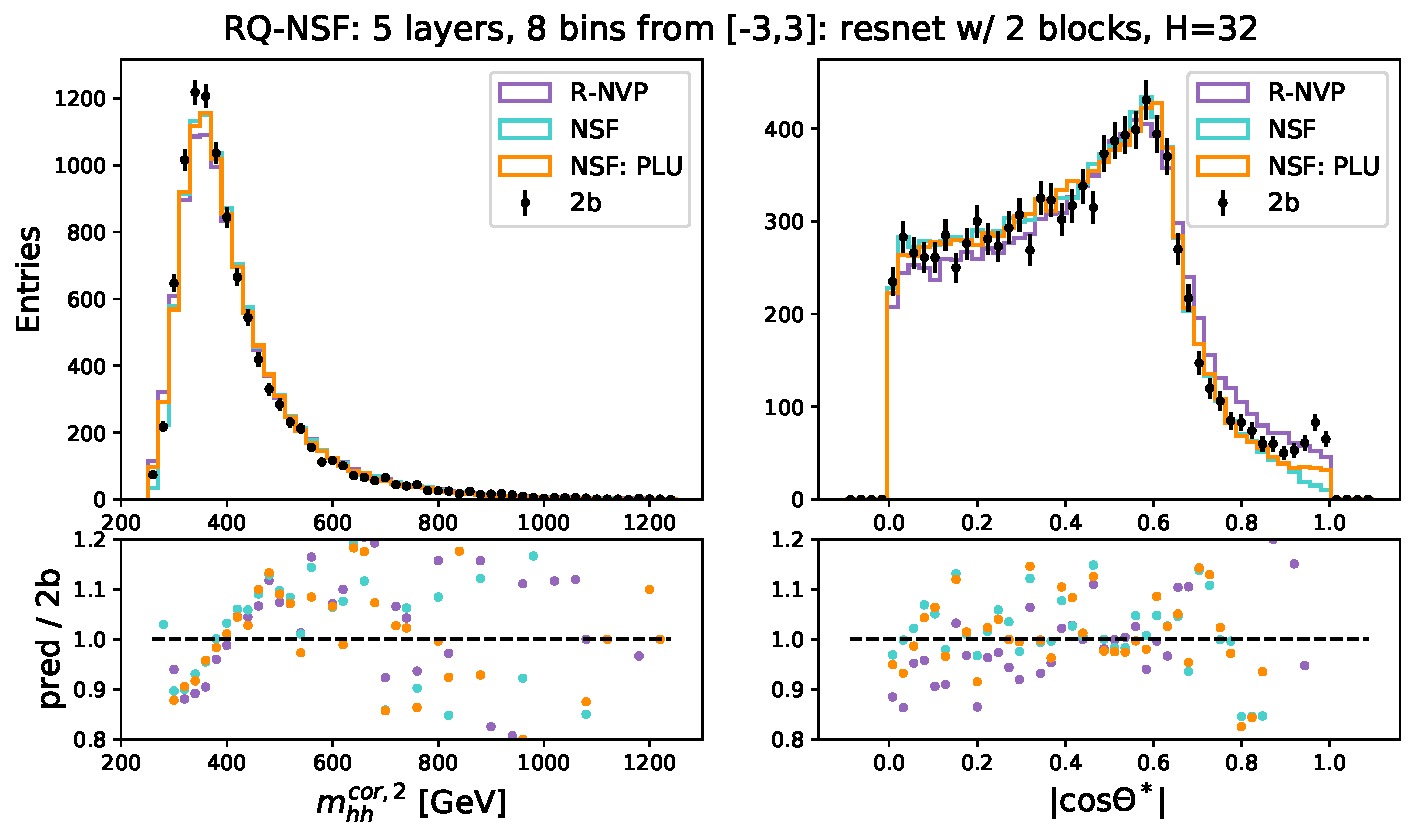
\includegraphics[width=\textwidth]{figures/flows/data16_PFlow-FEB20-5jets_SM_2b_p_0.01_2b_detaCut/nsf_rq-coupling_log_pT_h1_log_pT_h2_eta_h1_eta_h2_log_dphi_hh_random_5_layers_H_32_2_blocks_K_8_B_3_lr_0.001_0.001_iter0/m_hh_cor2_absCosThetaStar_cf_rnvp_lu.pdf}
\caption{}
\label{subsec:hp-modelChoice}
\end{figure}

\subsection{Hyperparameter optimization}
\label{subsec:hpOpt}


The rational quadratic neural spline flow paper considered modeling a range of applications from  the UCI dataset, so we used a range of hyperparameters that seemed to give good performance on the datasets with a similar number of training examples (see Table 4 of \cite{1906.04032}).

I considered B=3 (i.e, the rational qudratic spline transform is defined for the variable from (-3,3), and a simple linear transform \hl{or is this the identity} is used outside of this range.  To keep the inputs in the range where the nsf will have a meaningful transformation, abatch normalization layer was included after each of the flow steps. We didn't consider annealing the learning rate or gradient clipping even though this was used for the experiments in \cite{1906.04032} since we had good enough performance for our application before trying to include this - although testing the impact of this could be an interesting study in the future.

The choices for hyperparameters that I was considering were:

\begin{table}
\centering
\label{tab:hp-grid-search}
\begin{tabular}{|c|c|}
\toprule
%{} & \multicolumn{2}{c}{variable range} & \multicolumn{2}{c}{r} \\
Parameter range & parameter description  \\
\midrule
L = [5, 10] & number of layers (or flow steps) \\
K = [4,8] & number of knots in each spline transformation \\
$\alpha$ = 3e-4, 5e-4,1e-3 & learning rate (for adam optimizer) \\
$p = 0, 0.1, 0.2$ & dropout fraction \\
$\beta$ = 0, 1e-6, 1e-5, 1e-4, 1e-3 & L2 regularization weight. \\ %The loss function is a sum of two terms: $\mathcal{L} = - \mathbb{E}p\sim \text{data} \left[ p_flow \right] + \beta \sum_i |w_i |^2$ \\
num\_blocks = 1,2 & The number of blocks for the res net predicting the spline parameters \\
H = 16,32, 64 & hidden dimensions of the nns. \\
\bottomrule
\end{tabular}
\caption{Hyperparameters ranges considered for the random search.}
\end{table}

We did a random search over the hyper parameters to train 90 different configurations, where each configuration choice was trained 25 times.

\subsection{Choice of metric}
\label{subsec:hp-metric}

\def\figpath{figures/flows/data16_PFlow-FEB20-5jets_SM_2b_p_0.01_2b_detaCut/nsf_rq-coupling_log_pT_h1_log_pT_h2_eta_h1_eta_h2_log_dphi_hh_lu_hpScan}

\begin{figure}
\centering
\subfloat[SR loss]{
	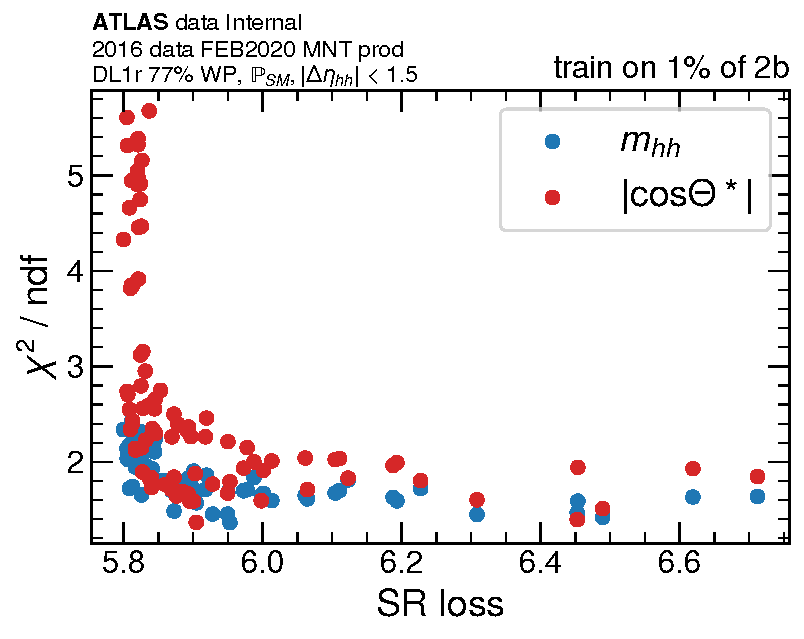
\includegraphics[width=0.44\textwidth]{{\figpath/chi2ndf_m_hh_absCosThetaStar_vs_SR_loss.pdf}}
	\label{fig:sr-loss}
	}
\subfloat[Loss on the validation set.]{
	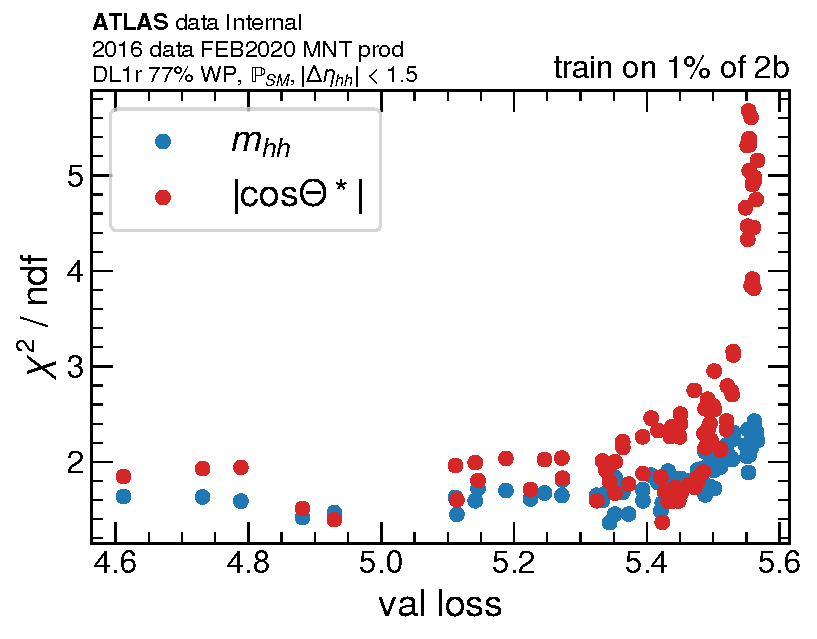
\includegraphics[width=0.44\textwidth]{{\figpath/chi2ndf_m_hh_absCosThetaStar_vs_val_loss.pdf}}
	\label{fig:val-loss}
	}
\caption{To choose the optimal model we found that minimizing the validation loss was a better metric than minimizing the SR loss.}
\label{fig:metric-choice}
\end{figure}




%\subsection{Training years together}
%\label{subsec:yrInclTraining}